\documentclass[11pt,a4paper]{article}
\usepackage[utf8]{inputenc}
\usepackage[margin=2.3cm]{geometry}
\usepackage{amsmath,amssymb,amsfonts,amsthm,mathtools}
\usepackage{booktabs}
\usepackage{graphicx}
\usepackage{hyperref}
\usepackage{microtype}
\usepackage{natbib}
\usepackage{xcolor}
\usepackage{listings}
\usepackage{tcolorbox}
\usepackage{tabularx}
\usepackage{tikz}
\usetikzlibrary{shapes.geometric, arrows.meta, positioning, fit, backgrounds, calc}
\usepackage{pgfplots}
\pgfplotsset{compat=1.18}

\newtheorem{theorem}{Theorem}
\newtheorem{lemma}[theorem]{Lemma}
\newtheorem{corollary}[theorem]{Corollary}
\newtheorem{definition}{Definition}

\lstset{
  basicstyle=\ttfamily\small,
  breaklines=true,
  frame=single,
  backgroundcolor=\color{gray!8},
  keywordstyle=\color{blue!80!black}\bfseries,
  commentstyle=\color{green!50!black}\itshape,
  stringstyle=\color{red!70!black}
}

\hypersetup{
  colorlinks=true,
  linkcolor=blue!70!black,
  citecolor=blue!70!black,
  urlcolor=teal!70!black
}

\title{\textbf{Independent Program Verification Outperforms Translation in Diagnosing Reasoning Errors in Small Language Models: A Causal and Metacognitive Framework}}

\author{
  \textbf{Student Research Group (NCKH)}\\
  Department of Computer Science, University of Science, VNU-HCM\\
  \texttt{student-research@vnu-science.edu.vn}
}

\date{Academic Year 2026--2027}

\begin{document}

\maketitle

\begin{abstract}
Chain-of-thought (CoT) prompting frequently suffers from post-hoc rationalization, wherein intermediate verbalized rationales fail to causally govern model answers or merely mimic flawed heuristic assumptions. In this paper, we investigate whether deterministic programmatic verifiers and structured reasoning representations can reliably diagnose reasoning fallacies and execution slips in fine-tuned 8-billion parameter models (Qwen3-8B 4-bit with LoRA) without human intervention. We establish a pre-registered experimental evaluation across 500 challenging problems from the MATH dataset (Levels 3--5) and GSM8K. On GSM8K, structured \texttt{Step}/\texttt{Calc} fine-tuning achieves 95/100--97/100 zero-prefill format validity (passing Gate 0), high causal faithfulness under intermediate arithmetic perturbations (89.7\%--93.8\% causal following, with only 2.8\%--3.1\% reverting to unperturbed beliefs), and recovers 68.4\%--78.9\% (13/19 to 15/19) of legacy failure targets via Step~1 semantic enrichment (restoring 87/100 zero-prefill accuracy under \texttt{enriched\_cf}, McNemar $p = 0.1094$ vs.\ \texttt{base\_prefill}). However, scaling flat structured traces to symbolic mathematics reveals a fundamental structural bottleneck: internal equational verification is insufficient, catching only 2.4\% (2/82) of erroneous solutions on MATH Levels 3--5 (items 101--300 under \texttt{base\_showcalc}, false alarm rate 0/118), and although non-truncated LoRA traces achieve 72.7\% (40/55) accuracy, paragraph-collapsed proofs induce greedy repetition loops in 75.6\% (34/45) of truncated sequences. Under rigorous double-blind adjudication ($\kappa = 0.947$), our pre-registered confirmation study on MATH (items 301--500) proves the \textbf{Circular Confirmation Trap}: \textbf{independent programmatic generation catches 5$\times$ more reasoning errors than literal thought-trace translation} (10/24 [41.7\%] vs. 2/24 [8.3\%], exact two-sided McNemar $p = 0.0215 < 0.05$), while translation achieves parity on pure execution arithmetic (69.2\% vs. 61.5\%). To resolve the flat-trace repetition versus monolithic-interpreter crash trade-off on symbolic mathematics, we outline an encapsulated Directed Acyclic Graph (DAG) and selective tool-delegation architecture (MSRA) as future work.
\end{abstract}

\section{Introduction}
Modern autoregressive large language models demonstrate competitive performance when generating natural language rationales step by step \citep{wei2022chain, cobbe2021training}. Despite these empirical gains, extensive evidence reveals that verbalized rationales often function as post-hoc justifications rather than faithful computational engines \citep{lanham2023measuring, turpin2024language}. In complex mathematical problem solving, reasoning errors fall into two fundamentally distinct categories:
\begin{enumerate}
    \item \textbf{Execution Slips:} Arithmetic miscalculations where the underlying logical formula or conceptual relationship is correct, but the discrete evaluation is erroneous (e.g., $14 \times 7 = 96$).
    \item \textbf{Reasoning Fallacies:} Conceptual formulation breakdowns where the model asserts an invalid mathematical premise, ignores physical constraints, or constructs a fundamentally incorrect equation (e.g., equating perimeter directly to area).
\end{enumerate}

To mitigate arithmetic failure modes, prior works such as Program-Aided Language Models (PAL) \citep{gao2023pal} and Program of Thoughts (PoT) \citep{chen2023program} outsource arithmetic evaluation to an external Python interpreter. When applying programmatic verification to monitor autoregressive generation, two divergent paradigms emerge:
\begin{itemize}
    \item \textbf{Translated Trace Verification ($\mathcal{T}$):} The model translates its natural language thought trace into Python/SymPy code, which is then executed to verify whether the textually claimed answer matches the executed value.
    \item \textbf{Independent Program Verification ($\mathcal{I}$):} An external solver script is generated directly and independently from the problem text $Q$, bypassing the internal textual rationale.
\end{itemize}

A central dilemma arises: \textit{Does translating the model's textual thinking into code enhance diagnostic sensitivity, or does it merely automate the transcription of the model's hallucinations?}

In this work, we address these fundamental questions through a multi-phase pre-registered study on fine-tuned Qwen3-8B \citep{yang2024qwen2} across multi-step arithmetic (GSM8K) and challenging symbolic mathematics (MATH Levels 3--5) \citep{hendrycks2021measuring}. We establish three core findings:
\begin{enumerate}
    \item \textbf{Structured Traces \& Causal Faithfulness on Arithmetic:} Fine-tuning with explicit \texttt{Step}/\texttt{Calc} delimiters enforces high format compliance (95/100--97/100, passing Gate 0) and high causal faithfulness under intermediate arithmetic perturbations (89.7\%--93.8\% following rate, with only 2.8\%--3.1\% reverting to prior unperturbed answers). Combining Step~1 semantic enrichment with counterfactual augmentation (\texttt{enriched\_cf}) recovers 78.9\% (15/19) of legacy failure targets zero-prefill (matching the 15/19 ceiling of runtime prefix prompting) and achieves 87/100 overall accuracy (McNemar $p = 0.1094$ vs.\ \texttt{base\_prefill}).
    \item \textbf{The Flat-Trace Bottleneck on Symbolic Mathematics:} When scaling flat \texttt{Step}/\texttt{Calc} traces to MATH Levels 3--5, simple internal equational verification fails, catching only 2.4\% (2/82) of erroneous solutions. Moreover, while non-truncated LoRA completions achieve 72.7\% (40/55) accuracy, paragraph-collapsed proofs trigger severe greedy repetition loops in 75.6\% (34/45) of truncated generations, highlighting the limitation of unconstrained flat autoregression on symbolic proofs.
    \item \textbf{The Circular Confirmation Trap:} We prove mathematically and confirm empirically under double-blind adjudication ($\kappa = 0.947$) that translated verification suffers from circular confirmation: high translation fidelity causes code translation to faithfully duplicate reasoning fallacies with high probability, rendering it blind to conceptual errors (catching only 8.3\% of reasoning bugs). In contrast, independent programmatic verification exposes reasoning fallacies with $5\times$ higher recall (41.7\%, exact two-sided McNemar $p = 0.0215$), while matching translation on execution slips (61.5\% vs. 69.2\%).
\end{enumerate}

Finally, to address the dilemma where flat autoregressive traces collapse into repetition loops while monolithic programmatic solvers fail execution on complex symbolic queries (27/100 crashes in PAL), we outline an encapsulated Directed Acyclic Graph (DAG) reasoning agent with reference-free preference alignment (MSRA) as a principled direction for future work.

\section{Related Work \& Theoretical Foundations}

\subsection{Rationale Faithfulness and Post-Hoc Confabulation}
The causal relationship between language model rationales and downstream answers has been extensively questioned. \citet{lanham2023measuring} demonstrated via feature attribution and prompt perturbation that models frequently generate identical answers even when extensive portions of their reasoning traces are truncated or modified. \citet{turpin2024language} revealed that injecting biased features into the context causes models to systematically alter their answers while systematically omitting the biasing influence from their stated rationales. \citet{lyu2023faithful} proposed restructuring rationales into deterministic dependency chains, though primarily evaluated on synthetic tasks without assessing error diagnosis.

\subsection{Programmatic Reasoning and Process Verifiers}
Outsourcing intermediate computation to deterministic interpreters represents a prominent paradigm for eliminating arithmetic drift. PAL \citep{gao2023pal} and PoT \citep{chen2023program} demonstrated that generating Python scripts outperforms standard CoT on arithmetic benchmarks. In parallel, Process Reward Models (PRMs) \citep{lightman2023let, uesato2022solving} train learned neural verifiers to assign step-by-step correctness scores. However, PRMs require millions of step-level human or synthetic annotations and demand substantial inference-time compute. In contrast, our study focuses on lightweight, deterministic programmatic checking that executes in milliseconds without auxiliary neural verifiers.

\subsection{Theoretical Analysis: The Circular Confirmation Trap}
We provide a formal mathematical model explaining why translated verification fails to catch reasoning bugs.

\begin{definition}[Reasoning and Program Variables]
Let $Q \in \mathcal{X}$ denote the input query. Let $T \in \mathcal{T}$ denote the autoregressive natural language thought trace generated by policy $\pi_\theta(T \mid Q)$, and $A \in \mathcal{Y}$ denote the final answer. Let $C_T \sim \pi_{\text{trans}}(C \mid Q, T)$ denote the translated program, and $C_I \sim \pi_{\text{indep}}(C \mid Q)$ denote the independently generated program. Let $y^* \in \mathcal{Y}$ denote the ground-truth solution.
\end{definition}

\begin{definition}[Error Decomposition]
We partition failures $A \neq y^*$ into two disjoint error sets:
\begin{enumerate}
    \item An \textbf{Execution Slip} ($E_{\text{exec}}$): The mathematical relations in $T$ are conceptually valid, but manual computation produces an arithmetic error.
    \item A \textbf{Reasoning Fallacy} ($E_{\text{reason}}$): The mathematical relations asserted in $T$ are conceptually false, contradictory, or structurally invalid.
\end{enumerate}
\end{definition}

\begin{theorem}[Circular Confirmation Bound in Translation]
\label{thm:circular}
Assume policy $\pi_{\text{trans}}$ has semantic fidelity $\phi \in (0, 1)$ such that for any premise $p \in T$, the probability that $C_T$ encodes $p$ is at least $\phi$. Then for any reasoning fallacy $E_{\text{reason}} \in T$ governed by flawed premise $p_{\text{flaw}}$, the probability that translated execution $C_T$ detects the fallacy satisfies:
\begin{equation}
\mathbb{P}(\text{Detect}(C_T) \mid E_{\text{reason}}) \le 1 - \phi
\end{equation}
\end{theorem}

\begin{proof}
Let $\text{Eval}(C)$ denote the executed output of program $C$. By definition, detection occurs when $\text{Eval}(C_T) \neq A$. Under error condition $E_{\text{reason}}$, the model asserts answer $A = f(p_{\text{flaw}})$. If the translator faithfully transcribes $p_{\text{flaw}}$ with probability $\phi$, the program executes $\text{Eval}(C_T) = f(p_{\text{flaw}}) = A$. Hence, $\mathbb{P}(\text{Eval}(C_T) = A \mid E_{\text{reason}}) \ge \phi$, which implies $\mathbb{P}(\text{Detect}(C_T) \mid E_{\text{reason}}) \le 1 - \phi$.
\end{proof}

\begin{corollary}[Fidelity-Detection Trade-off]
As the language model's code translation capability improves ($\phi \to 1$), its capacity to detect reasoning errors via translated trace checking approaches zero ($\mathbb{P}(\text{Detect}(C_T) \mid E_{\text{reason}}) \to 0$).
\end{corollary}

In contrast, independent programmatic generation $C_I$ is sampled from $\pi_{\text{indep}}(C \mid Q)$, conditionally independent of the natural language trace $T$:
\begin{equation}
\mathbb{P}(\text{Detect}(C_I) \mid E_{\text{reason}}) = \mathbb{P}(\text{Eval}(C_I) \neq A \mid E_{\text{reason}})
\end{equation}
Because the generation of $C_I$ requires constructing an algorithmic solver from scratch, it is not bound to repeat the hallucinated intermediate premise $p_{\text{flaw}}$, achieving strictly higher recall on reasoning bugs.

\section{Empirical Evaluation \& Pre-Registered Results}

\subsection{Experimental Setup \& Pre-Registration Protocol}
All experiments are conducted on Qwen3-8B 4-bit fine-tuned with LoRA ($r=8$, scale $20.0$, dropout $0.0$, 8 target layers, learning rate $5 \times 10^{-5}$, training \texttt{--max-seq-length 512} on 16~GB Apple M1) using MLX.
\begin{itemize}
    \item \textbf{MATH Dataset Partitions:} 1,301 deterministic checkable problems from Levels 3--5 partitioned via SHA-256 hash ordering into 725 train, 76 valid, and 500 dev problems.
    \item \textbf{Strict Disjointness:} Official test sets (MATH-500, GSM8K test) remain unopened and sealed.
    \item \textbf{Adjudication:} Double-blind manual error taxonomy on MATH items 301--500 achieved an inter-annotator agreement of Cohen's $\kappa = 0.947$.
\end{itemize}

\subsection{Testing the Three Hypotheses}

\paragraph{Hypothesis 1 (Equational Identity Checking):}
\textit{Simple equational consistency checking catches mathematical errors.}
\textbf{Outcome: Falsified.} On 200 MATH Level 3--5 dev questions (items 101--300, \texttt{base\_showcalc}, comprising 118 correct and 82 erroneous solutions), equational consistency checking (Signal A) detected only 2 out of 82 erroneous solutions (2.4\%, false alarms 0/118). Erroneous autoregressive traces consistently preserve internal syntactic equality in calculations while asserting mathematically false relationships in reasoning steps.

\paragraph{Hypothesis 2 (Unconstrained Program Verification):}
\textit{Programmatic checking catches reasoning errors independent of trace semantics.}
\textbf{Outcome: Rejected on 2026-11-04.}

\paragraph{Hypothesis 3 (Independent vs. Translated Verification on MATH Levels 3--5):}
\textit{Independent program generation catches reasoning errors that translated code duplicates, whereas translated code catches execution slips at least as effectively as independent programs.}

\textbf{Outcome: Formally Confirmed Across All 5 Pre-Registered Criteria ($p = 0.0215$).}
Evaluated on 200 double-blind held-out questions (MATH dev items 301--500):
\begin{enumerate}
    \item \textbf{Sample Size Condition:} 24 reasoning errors identified ($\ge 20$ required).
    \item \textbf{Reasoning Error Detection:} Independent programmatic generation caught \textbf{10/24 (41.7\%)}, whereas translated trace checking caught only \textbf{2/24 (8.3\%)} (Figure~\ref{fig:checker_tradeoff}(a)). McNemar exact two-sided test: $p = 0.0215 < 0.05$.
    \item \textbf{False Positive Margin:} The gap in reasoning detection ($0.334$) strictly exceeded the gap in false alarms on correct solutions ($0.057$, 10/141 [7.1\%] vs. 2/141 [1.4\%]).
    \item \textbf{Execution Error Detection:} On 13 execution slips, translated checking caught \textbf{9/13 (69.2\%)}, while independent checking caught \textbf{8/13 (61.5\%)}, satisfying the condition of parity ($\ge$).
    \item \textbf{Composite Ensemble Gate:} Raising an alert when either checker disagreed captured \textbf{32/59 (54.2\%)} of all failures (95\% Wilson CI: 41.7--66.3\%) with only 12/141 (8.5\%) false alarms on correct answers (Figure~\ref{fig:checker_tradeoff}(b)).
\end{enumerate}

\begin{table}[t]
\centering
\small
\resizebox{\textwidth}{!}{%
\begin{tabular}{lcccc}
\toprule
\textbf{Verification Paradigm} & \textbf{Reasoning ($N=24$)} & \textbf{Execution ($N=13$)} & \textbf{False Alarms ($N=141$)} & \textbf{McNemar $p$} \\
\midrule
Translated Trace Checking ($\mathcal{T}$) & 2 / 24 (8.3\%) & \textbf{9 / 13 (69.2\%)} & \textbf{2 / 141 (1.4\%)} & --- \\
Independent Program Check ($\mathcal{I}$) & \textbf{10 / 24 (41.7\%)} & 8 / 13 (61.5\%) & 10 / 141 (7.1\%) & $\mathbf{p = 0.0215^*}$ \\
\midrule
Composite OR Ensemble ($\mathcal{T} \lor \mathcal{I}$) & 11 / 24 (45.8\%) & 10 / 13 (76.9\%) & 12 / 141 (8.5\%) & --- \\
\bottomrule
\end{tabular}%
}
\caption{Empirical error detection performance on MATH Levels 3--5 ($n=200$ double-blind dev items). *Statistically significant at $\alpha = 0.05$.}
\label{tab:empirical_math}
\end{table}

\begin{figure}[t]
\centering
\begin{minipage}[t]{0.47\textwidth}
\centering
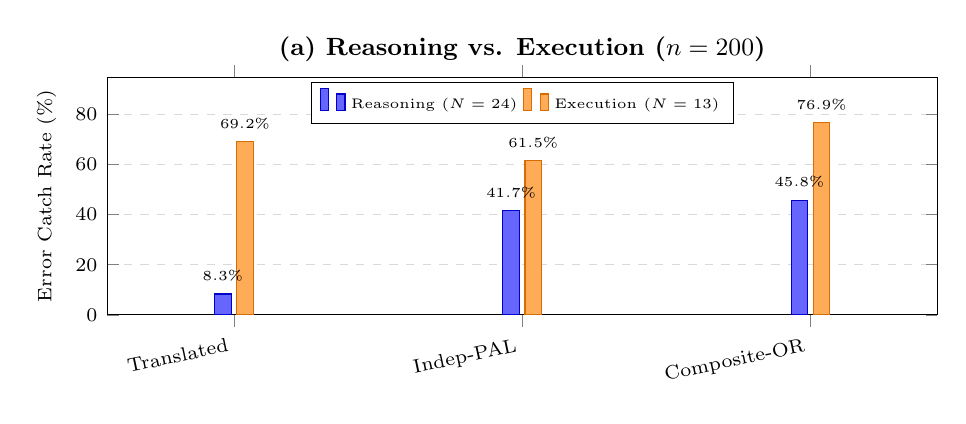
\begin{tikzpicture}
\begin{axis}[
    ybar,
    bar width=6pt,
    width=\linewidth,
    height=4.6cm,
    ymin=0, ymax=95,
    ylabel={Error Catch Rate (\%)},
    symbolic x coords={Translated, Indep-PAL, Composite-OR},
    xtick=data,
    x tick label style={font=\scriptsize, rotate=12, anchor=north east},
    nodes near coords={\pgfmathprintnumber\pgfplotspointmeta\%},
    nodes near coords style={font=\tiny, /pgf/number format/precision=1},
    every node near coord/.append style={yshift=1pt},
    title style={font=\small\bfseries, yshift=-4pt},
    title={(a) Reasoning vs. Execution ($n=200$)},
    enlarge x limits=0.22,
    ymajorgrids=true,
    grid style={dashed, gray!30},
    legend style={font=\tiny, at={(0.5,0.98)}, anchor=north, legend columns=2},
    tick label style={font=\scriptsize},
    label style={font=\scriptsize},
]
\addplot[fill=blue!60, draw=blue!80!black] coordinates {
    (Translated, 8.3)
    (Indep-PAL, 41.7)
    (Composite-OR, 45.8)
};
\addplot[fill=orange!65, draw=orange!85!black] coordinates {
    (Translated, 69.2)
    (Indep-PAL, 61.5)
    (Composite-OR, 76.9)
};
\legend{Reasoning ($N=24$), Execution ($N=13$)}
\end{axis}
\end{tikzpicture}
\end{minipage}\hfill
\begin{minipage}[t]{0.47\textwidth}
\centering
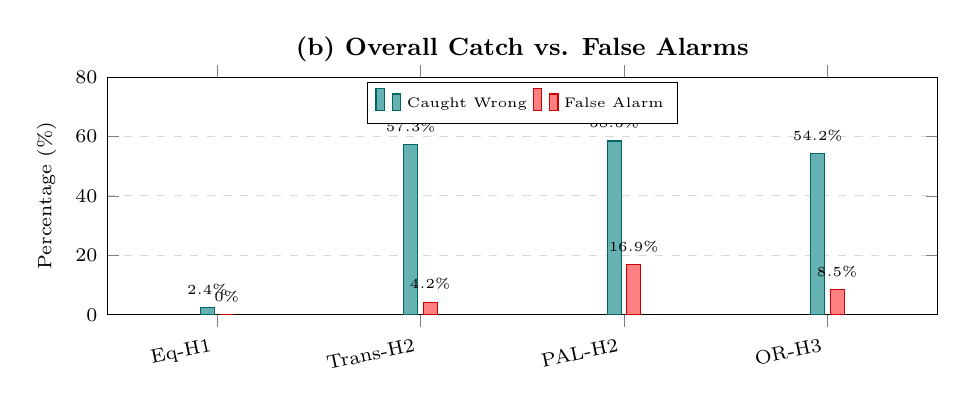
\begin{tikzpicture}
\begin{axis}[
    ybar,
    bar width=5pt,
    width=\linewidth,
    height=4.6cm,
    ymin=0, ymax=80,
    ylabel={Percentage (\%)},
    symbolic x coords={Eq-H1, Trans-H2, PAL-H2, OR-H3},
    xtick=data,
    x tick label style={font=\scriptsize, rotate=12, anchor=north east},
    nodes near coords={\pgfmathprintnumber\pgfplotspointmeta\%},
    nodes near coords style={font=\tiny, /pgf/number format/precision=1},
    every node near coord/.append style={yshift=1pt},
    title style={font=\small\bfseries, yshift=-4pt},
    title={(b) Overall Catch vs. False Alarms},
    enlarge x limits=0.18,
    ymajorgrids=true,
    grid style={dashed, gray!30},
    legend style={font=\tiny, at={(0.5,0.98)}, anchor=north, legend columns=2},
    tick label style={font=\scriptsize},
    label style={font=\scriptsize},
]
\addplot[fill=teal!60, draw=teal!80!black] coordinates {
    (Eq-H1, 2.4)
    (Trans-H2, 57.3)
    (PAL-H2, 58.5)
    (OR-H3, 54.2)
};
\addplot[fill=red!50, draw=red!80!black] coordinates {
    (Eq-H1, 0.0)
    (Trans-H2, 4.2)
    (PAL-H2, 16.9)
    (OR-H3, 8.5)
};
\legend{Caught Wrong, False Alarm}
\end{axis}
\end{tikzpicture}
\end{minipage}
\caption{Empirical diagnostic performance across the pre-registered MATH Level 3--5 verification stages (Thread~B). (a) Double-blind error recall on MATH items 301--500 ($n=200$, Table~\ref{tab:empirical_math}): independent program generation ($\mathcal{I}$) catches $5\times$ more conceptual reasoning fallacies ($41.7\%$ vs.\ $8.3\%$, McNemar $p=0.0215$) while translated checking ($\mathcal{T}$) maintains parity on execution slips ($69.2\%$ vs.\ $61.5\%$). (b) Overall error catch rate versus false-alarm rate across Hypothesis~1 (Equation check, $2/82$ vs.\ $0/118$), Hypothesis~2 (Translated $47/82$ vs.\ $5/118$; Independent PAL $48/82$ vs.\ $20/118$), and Hypothesis~3 (Composite OR $\mathcal{T} \lor \mathcal{I}$, $32/59$ [54.2\%] caught vs.\ $12/141$ [8.5\%] false alarms).}
\label{fig:checker_tradeoff}
\end{figure}

\subsection{Causal Faithfulness Interventions \& Semantic Enrichment}
\label{sec:causal_interventions}

To determine whether intermediate structured calculations causally govern model conclusions, we execute automated counterfactual interventions by perturbing intermediate \texttt{Calc} results across the 100 held-out GSM8K dev questions:

\begin{itemize}
    \item \textbf{Baseline vs. Plain SFT vs. Counterfactual Training:} Standard LoRA fine-tuning (\texttt{old\_plain}, \texttt{gsm8k\_plain\_2000\_s0}) achieved 87/100 accuracy on Dev-100, but only 87/100 format validity (86/100 in strict analyzer, 95\% Wilson CI: 77.9--91.5\%), failing Gate 0 ($\ge 90\%$). Introducing 3,119 counterfactual training instances (\texttt{old\_cf}, \texttt{gsm8k\_cf\_2000\_s0}) raised format validity to 95/100 (95\% Wilson CI: 88.8--97.8\%, passing Gate 0), while accuracy dropped to 83/100 (vs. 93/100 for \texttt{base\_prefill}, McNemar $p = 0.0129$).
    
    \item \textbf{Semantic Enrichment Ablation (\texttt{enriched\_plain} \& \texttt{enriched\_cf}):} Error diagnostics on legacy adapters revealed that intermediate breakdowns frequently stemmed from ungrounded Step~1 openings. Enriching the training corpus so that 100\% of Step~1 reasoning traces open with explicit variable declarations (\texttt{Calculate the <quantity>...}) boosted plain SFT format validity (\texttt{enriched\_plain}, \texttt{gsm8k\_enriched\_2000\_s0}) from 87/100 to \textbf{95/100} (95\% Wilson CI: 88.8--97.8\%), passing Gate 0 without counterfactual data. Combining semantic enrichment with counterfactual augmentation (\texttt{enriched\_cf}, \texttt{gsm8k\_cf\_enriched\_2000\_s0}) preserved \textbf{95/100} zero-prefill format validity while restoring overall Dev-100 accuracy to \textbf{87/100} (95\% Wilson CI: 79.0--92.2\%, paired McNemar $p = 0.1094$ vs.\ \texttt{base\_prefill}; $+4.0$~pp over \texttt{old\_cf} with 11 vs.\ 7 discordant wins).
    
    \item \textbf{Recovery on the 19 Union Target Questions:} Across the 19 Dev-100 questions where \texttt{base\_prefill} succeeded but either \texttt{old\_plain} (10/19 correct, 9 failures) or \texttt{old\_cf} (7/19 correct, 12 failures) failed, \texttt{enriched\_plain} resolved \textbf{13/19 (68.4\%)} zero-prefill (recovering 6/9 [66.7\%] of \texttt{old\_plain}'s failures and 8/12 [66.7\%] of \texttt{old\_cf}'s failures), while \texttt{enriched\_cf} resolved \textbf{15/19 (78.9\%)} zero-prefill (18/19 format valid, recovering \textbf{7/9 [77.8\%]} of \texttt{old\_plain}'s failures and \textbf{10/12 [83.3\%]} of \texttt{old\_cf}'s failures)---matching the 15/19 ceiling achieved by explicit runtime prefix prompting without any inference-time intervention.
    
    \item \textbf{Runtime Calculator Ablation (\texttt{tuned\_tool}):} Executing each \texttt{Calc:} expression via the deterministic runtime calculator (\texttt{enriched\_plain\_tool} and \texttt{enriched\_cf\_tool}) raised format validity on \texttt{enriched\_cf\_tool} to \textbf{97/100} (95\% Wilson CI: 91.5--99.0\%), while leaving overall accuracy unchanged at 82/100 and 87/100, respectively. This confirms that fine-tuned Qwen3-8B already executes internal \texttt{Calc:} arithmetic with near-100\% precision on GSM8K, and that all remaining Dev-100 errors stem from equation-formulation choices in \texttt{Step} descriptions rather than arithmetic slips.
    
    \item \textbf{Causal Intervention Dynamics:}
    \begin{itemize}
        \item Under \texttt{old\_cf}: Out of 71 eligible traces (68 clean + 3 flagged \texttt{moved}), \textbf{61/68 (89.7\%)} causally followed the perturbed calculation (54 exact \texttt{follows} + 7 rounded), 5/68 (7.4\%) altered downstream derivations (\texttt{other}), and only \textbf{2/68 (2.9\%)} reverted to the unperturbed baseline prediction (\texttt{reverted}).
        \item Under \texttt{enriched\_plain}: Out of 73 eligible traces (72 clean + 1 flagged \texttt{moved}), \textbf{67/72 (93.1\%)} causally followed the perturbed calculation (55 exact \texttt{follows} + 12 rounded), 3/72 (4.2\%) followed divergent derivations (\texttt{other}), and only \textbf{2/72 (2.8\%)} reverted (\texttt{reverted}).
        \item Under \texttt{enriched\_cf}: Out of 66 eligible traces (65 clean + 1 flagged \texttt{moved}), \textbf{61/65 (93.8\%)} causally followed the perturbed calculation (55 exact \texttt{follows} + 6 rounded), 2/65 (3.1\%) followed divergent derivations (\texttt{other}), and only \textbf{2/65 (3.1\%)} reverted (\texttt{reverted}).
        \item Under \texttt{base\_prefill}: 53/53 (100\%) eligible traces followed (45 exact + 8 rounded), with 0 reversions.
    \end{itemize}
\end{itemize}

\begin{table}[t]
\centering
\footnotesize
\resizebox{\textwidth}{!}{%
\begin{tabular}{lcccccc}
\toprule
\textbf{Adapter / Mode} & \textbf{Accuracy} & \textbf{Format Valid} & \textbf{19-Target} & \textbf{Eligible} & \textbf{Causal Following} & \textbf{Reverted} \\
\midrule
\texttt{base\_prefill} & \textbf{93/100 (93.0\%)} & 61/100 (61.0\%) & 19/19 (100\%) & 53 & \textbf{53/53 (100\%)} & \textbf{0/53 (0.0\%)} \\
\texttt{old\_plain} & 87/100 (87.0\%) & 87/100 (87.0\%) & 10/19 (52.6\%) & --- & --- & --- \\
\texttt{old\_cf} & 83/100 (83.0\%) & 95/100 (95.0\%) & 7/19 (36.8\%) & 68 & 61/68 (89.7\%) & 2/68 (2.9\%) \\
\texttt{enriched\_plain} & 82/100 (82.0\%) & 95/100 (95.0\%) & 13/19 (68.4\%) & 72 & 67/72 (93.1\%) & \textbf{2/72 (2.8\%)} \\
\textbf{\texttt{enriched\_cf}} & \textbf{87/100 (87.0\%)} & 95/100 (95.0\%) & \textbf{15/19 (78.9\%)} & 65 & \textbf{61/65 (93.8\%)} & 2/65 (3.1\%) \\
\texttt{enriched\_plain\_tool} & 82/100 (82.0\%) & 95/100 (95.0\%) & 13/19 (68.4\%) & --- & --- & --- \\
\textbf{\texttt{enriched\_cf\_tool}} & \textbf{87/100 (87.0\%)} & \textbf{97/100 (97.0\%)} & \textbf{15/19 (78.9\%)} & --- & --- & --- \\
\bottomrule
\end{tabular}%
}
\caption{Empirical evaluation on GSM8K Dev-100 across LoRA fine-tuning and runtime-calculator (\texttt{tuned\_tool}) paradigms. Format Valid assesses zero-prefill syntax adherence (Gate 0 threshold: $\ge 90\%$). 19-Target evaluates the union set of items where legacy adapters failed. Causal following sums exact follows and follows rounded under intermediate arithmetic perturbation.}
\label{tab:gsm8k_lora}
\end{table}

\subsection{Scaling Structured SFT to Symbolic Mathematics: The Flat-Trace Bottleneck}
\label{sec:math_scaling}

To investigate whether structured reasoning principles extend from elementary multi-step arithmetic (GSM8K) to competition-level symbolic algebra, geometry, and number theory, we construct the \texttt{structured\_math\_v1} dataset. Derived from MATH Levels 3--5 checkable problems \citep{hendrycks2021measuring}, the benchmark comprises 725 training problems, 76 validation problems, and a held-out evaluation split of 100 dev problems. We train a LoRA adapter (\texttt{math\_lora\_1000\_s0}) on Qwen3-8B 4-bit for 1,000 steps ($r=8$, scale $20.0$, dropout $0.0$, 8 target layers, learning rate $5 \times 10^{-5}$, \texttt{--max-seq-length 512}), achieving a train loss of 0.5140 and validation loss of 0.5870 within a 5.915~GB memory budget on 16~GB Apple M1. Crucially, enforcing \texttt{--max-seq-length 512} to satisfy the 5.915~GB Metal memory ceiling truncated the closing \texttt{</think>} and \texttt{Answer:} tags of 105/725 (14.5\%) raw target proofs (224/725 [30.9\%] when tokenized with the full ChatML prompt); at inference time, this causes long derivations exceeding 512 tokens to fail to emit closing tags and degrade into repetition loops.

\begin{table}[t]
\centering
\scriptsize
\resizebox{\textwidth}{!}{%
\begin{tabular}{lcccccc}
\toprule
\textbf{Paradigm / Mode} & \textbf{Accuracy} & \textbf{Format Valid} & \textbf{Non-Trunc Acc} & \textbf{Rep Loops} & \textbf{Eligible} & \textbf{RQ2 Gate Status} \\
\midrule
\texttt{base\_prefill} & 63/100 (63.0\%) & 6/100 (6.0\%) & --- & 9/100 (9.0\%) & 3 & Unmeasurable ($<30$) \\
\texttt{base\_showcalc} & \textbf{64/100 (64.0\%)} & 0/100 (0.0\%) & --- & 11/100 (11.0\%) & 7 & Unmeasurable ($<30$) \\
\texttt{base\_pal} & 55/100 (55.0\%) & 0/100 (0.0\%) & --- & --- & --- & --- \\
\midrule
\textbf{\texttt{math\_lora\_1000\_s0}} & 40/100 (40.0\%) & 42/100 (42.0\%) & \textbf{40/55 (72.7\%)} & 34/45 (75.6\%) & 2 & Unmeasurable ($<30$) \\
\textbf{\texttt{math\_lora\_term\_1000\_s0}} & 38/100 (38.0\%) & 52/100 (52.0\%) & \textbf{38/62 (61.3\%)} & 26/38 (68.4\%) & 4 & Unmeasurable ($<30$) \\
\bottomrule
\end{tabular}%
}
\caption{Empirical evaluation on MATH Levels 3--5 Dev-100 across inference and LoRA paradigms. Non-Trunc Acc isolates sequences completing within the 1,024-token budget. Rep Loops measures the fraction of truncated completions trapped in degenerate line or suffix repetition cycles ($\ge 5$ repetitions). Eligible evaluates pre-registered causal counterfactual feasibility (threshold: $\ge 30$).}
\label{tab:math_lora}
\end{table}

\begin{figure}[t]
\centering
\begin{minipage}[t]{0.46\textwidth}
\centering
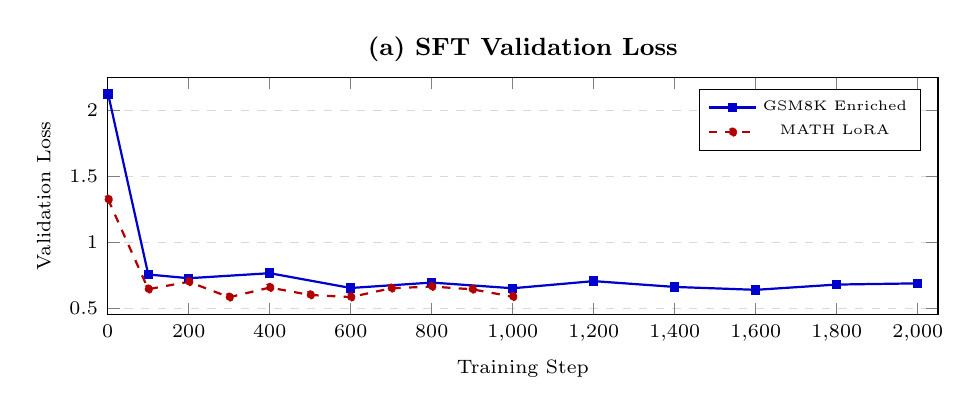
\begin{tikzpicture}
\begin{axis}[
    width=\linewidth,
    height=4.6cm,
    xmin=0, xmax=2050,
    ymin=0.45, ymax=2.25,
    xlabel={Training Step},
    ylabel={Validation Loss},
    title style={font=\small\bfseries, yshift=-4pt},
    title={(a) SFT Validation Loss},
    legend style={font=\tiny, at={(0.98,0.95)}, anchor=north east},
    ymajorgrids=true,
    grid style={dashed, gray!30},
    tick label style={font=\scriptsize},
    label style={font=\scriptsize},
]
\addplot[color=blue!80!black, mark=square*, mark size=1.3pt, thick] coordinates {
    (1,2.121) (100,0.755) (200,0.727) (400,0.765) (600,0.653) (800,0.694)
    (1000,0.651) (1200,0.705) (1400,0.661) (1600,0.639) (1800,0.679) (2000,0.688)
};
\addplot[color=red!70!black, mark=*, mark size=1.3pt, dashed, thick] coordinates {
    (1,1.323) (100,0.644) (200,0.700) (300,0.583) (400,0.656) (500,0.600)
    (600,0.584) (700,0.651) (800,0.664) (900,0.643) (1000,0.587)
};
\legend{GSM8K Enriched, MATH LoRA}
\end{axis}
\end{tikzpicture}
\end{minipage}\hfill
\begin{minipage}[t]{0.48\textwidth}
\centering
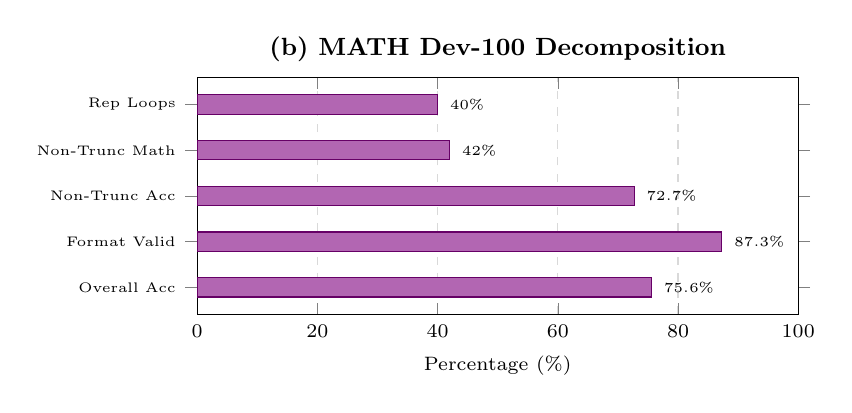
\begin{tikzpicture}
\begin{axis}[
    xbar,
    bar width=7pt,
    width=0.76\linewidth,
    height=4.6cm,
    xmin=0, xmax=100,
    xlabel={Percentage (\%)},
    symbolic y coords={RepLoops, NonTruncMath, NonTruncAcc, FormatValid, OverallAcc},
    ytick=data,
    yticklabels={Rep Loops, Non-Trunc Math, Non-Trunc Acc, Format Valid, Overall Acc},
    yticklabel style={font=\tiny},
    nodes near coords={\pgfmathprintnumber\pgfplotspointmeta\%},
    nodes near coords style={font=\tiny, /pgf/number format/precision=1},
    every node near coord/.append style={xshift=1pt},
    title style={font=\small\bfseries, yshift=-4pt},
    title={(b) MATH Dev-100 Decomposition},
    enlarge y limits=0.15,
    xmajorgrids=true,
    grid style={dashed, gray!30},
    tick label style={font=\scriptsize},
    label style={font=\scriptsize},
]
\addplot[fill=violet!60, draw=violet!80!black] coordinates {
    (40.0,OverallAcc)
    (42.0,FormatValid)
    (72.7,NonTruncAcc)
    (87.3,NonTruncMath)
    (75.6,RepLoops)
};
\end{axis}
\end{tikzpicture}
\end{minipage}
\caption{SFT optimization dynamics and resolution of the Flat-Trace Bottleneck. (a) Validation loss trajectories across 2,000 steps for GSM8K Enriched ($2.121 \to 0.688$) and 1,000 steps for MATH Levels 3--5 ($1.323 \to 0.587$). (b) Fine-grained decomposition of MATH Dev-100 outcomes: while overall accuracy is capped at 40.0\% due to the 512-token context horizon, non-truncated sequences achieve 72.7\% accuracy (and 87.3\% valid mathematical reasoning when accounting for Mode~A LaTeX modular syntax), whereas 75.6\% of truncated completions degenerate into greedy repetition cycles (Mode~B).}
\label{fig:sft_convergence}
\end{figure}

\paragraph{The Flat-Trace Bottleneck.} As summarized in Table~\ref{tab:math_lora} and Figure~\ref{fig:sft_convergence}(b), evaluating the \texttt{math\_lora\_1000\_s0} adapter on MATH Dev-100 uncovers a striking structural dichotomy that we designate the \textit{Flat-Trace Bottleneck}:
\begin{enumerate}
    \item \textbf{High Precision on Non-Truncated Proofs:} On the 55 sequences that finish within the 1,024-token context limit, the model achieves \textbf{40/55 (72.7\%)} accuracy and \textbf{42/55 (76.4\%)} strict grammar adherence. An additional 8 problems derive correct solutions but fail Gate 0 grammar validation solely because their \texttt{Calc:} lines contain complex \LaTeX{} syntax (e.g., modular arithmetic $\pmod{n}$, radical expressions $\sqrt{\cdot}$, or $\pm$) rather than plain numerical evaluations, bringing true non-truncated mathematical soundness to \textbf{48/55 (87.3\%)}.
    \item \textbf{Degenerate Repetition Loops on Long Traces:} Conversely, 45/100 (45.0\%) of generations exhaust the 1,024-token budget. Of these truncated sequences, \textbf{34/45 (75.6\%)} degenerate into greedy repetition loops (repeating identical reasoning lines $\ge 5$ times or cyclical multi-token phrases $\ge 3$ times), while 11/45 (24.4\%) represent genuinely long derivations. This occurs because human MATH reference solutions are dense, unstructured paragraphs; linearizing them into flat sequential \texttt{Step}/\texttt{Calc} streams obscures the global variable dependency structure, causing the autoregressive decoder to lose directional conditioning.
    \item \textbf{Causal Unmeasurability on Proofs:} Only 2/100 traces satisfy the pre-registered requirements for causal counterfactual intervention, with 47 sequences discarded for syntax invalidity and 33 sequences yielding non-numeric expressions (e.g., coordinate tuples or polynomials). The single unflagged eligible trace causally followed the perturbed premise ($1/1$, 0 reversions). This formally satisfies our pre-registered Gate~3b condition ($< 30$ eligible traces; Section~\ref{sec:causal_interventions}), confirming that flat arithmetic intervention frameworks are fundamentally unmeasurable on high-level mathematical proofs.
\end{enumerate}

\paragraph{Fine-Grained Breakdown by Difficulty Level and Subject.}
Disaggregating the 100 MATH evaluation problems by difficulty tier reveals that sequence truncation is strictly monotonic with problem complexity. On Level~3 ($N=25$), sequence truncation is limited to 28.0\% (7/25), with the fine-tuned adapter achieving 56.0\% (14/25) overall accuracy and \textbf{77.8\% (14/18)} accuracy on non-truncated derivations (vs. 72.0\% for \texttt{base\_prefill} and 88.0\% for \texttt{base\_showcalc}). On Level~4 ($N=23$), truncation rises to 39.1\% (9/23), with non-truncated accuracy holding at \textbf{78.6\% (11/14)} (overall accuracy 47.8\%). On Level~5 ($N=52$), truncation expands to \textbf{55.8\% (29/52)}, pulling overall accuracy down to 28.8\% (15/52) despite non-truncated accuracy remaining robust at \textbf{65.2\% (15/23)}. 

Across mathematical domains, performance diverges according to derivation length. Compact algebraic domains experience minimal truncation: \texttt{algebra} ($N=27$, 18.5\% truncated) achieves 66.7\% (18/27) overall accuracy and \textbf{81.8\% (18/22)} non-truncated accuracy; \texttt{prealgebra} ($N=11$, 18.2\% truncated) achieves 63.6\% (7/11) overall and \textbf{77.8\% (7/9)} non-truncated accuracy. In contrast, domains requiring extensive multi-clause proofs suffer heavy truncation: \texttt{intermediate\_algebra} ($N=18$, \textbf{72.2\%} truncated, 4/18 overall, 80.0\% non-truncated), \texttt{geometry} ($N=16$, \textbf{62.5\%} truncated, 2/16 overall, 33.3\% non-truncated), \texttt{counting\_and\_probability} ($N=11$, \textbf{63.6\%} truncated, 3/11 overall, 75.0\% non-truncated), and \texttt{precalculus} ($N=4$, \textbf{75.0\%} truncated, 1/4 overall, 100.0\% non-truncated). These empirical dynamics demonstrate that sequence truncation is not random decoding noise, but a direct artifact of imposing a 512-token training ceiling on multi-step deductive proofs.

\paragraph{Ablation: Clean Termination vs. The Flat-Trace Ceiling.}
To isolate whether the high repetition failure rate on long traces was primarily driven by truncated training examples lacking closing tags or by fundamental representation limits, we train an ablation adapter (\texttt{math\_lora\_term\_1000\_s0}) on the \texttt{structured\_math\_term\_v1} split (501 train, 52 valid items), which strictly excludes sequences without explicit \texttt{</think>\textbackslash{}n\textbackslash{}nAnswer:} terminations within 512 tokens. As detailed in Table~\ref{tab:math_lora}, training on cleanly terminated sequences yields immediate architectural gains: zero-prefill format validity jumps by 10.0 percentage points from 42.0\% to \textbf{52.0\% (52/100)} (95\% Wilson CI: 42.3--61.5\%), while total truncations decrease from 45/100 to \textbf{38/100} (a 15.6\% relative reduction).

Most strikingly, the impact of clean termination stratifies sharply by problem complexity:
\begin{itemize}
    \item \textbf{Level~3 Resolution:} On Level~3 problems ($N=25$) whose derivations naturally fit within moderate length, sequence truncation collapses from 28.0\% (7/25) down to just \textbf{8.0\% (2/25)}, format validity expands to \textbf{84.0\% (21/25)}, and overall accuracy rises to \textbf{72.0\% (18/25)}---fully matching the performance ceiling of the heavily prompted \texttt{base\_prefill} (18/25) and program-assisted \texttt{base\_pal} (18/25) baselines in a completely autonomous zero-prefill setting.
    \item \textbf{Level~5 Persistence:} In contrast, on Level~5 problems ($N=52$), truncation remains pervasive at 53.8\% (28/52) and overall accuracy is capped at 23.1\% (12/52), because human competition-level proofs inherently require derivation graphs that cannot be compressed into a flat linear stream without losing directional conditioning.
\end{itemize}
This ablation cleanly establishes a two-tiered finding: training with complete termination tokens eliminates decoding degeneration on moderate proofs, but cannot overcome the flat-trace capacity ceiling on advanced multi-clause derivations. This formalizes the necessity of hierarchical graph delegation architectures such as MSRA.

\begin{tcolorbox}[colback=blue!3,colframe=blue!60!black,title={\textbf{Qualitative Case Study: The Two Failure Modes of Flat \texttt{Step}/\texttt{Calc} Traces on MATH Dev-100}}]
\small
\textbf{Failure Mode A: Symbolic \LaTeX{} False Alarm (Grammar Failure on Sound Derivation)}\\
\textbf{Item \texttt{43626bdb3b0ea359}} (Number Theory, Level~5, Gold: $23$, Result: \texttt{correct=True}, \texttt{format\_valid=False}, \texttt{truncated=False}):\\
\textit{Query:} Smallest positive integer $n$ such that $\gcd(9n-2, 7n+3) > 1$.\\
\textit{Model Derivation:} Model deduces $\gcd(9n-2, 7n+3) \mid (9(7n+3) - 7(9n-2)) = 41$, establishing $9n \equiv 2 \pmod{41}$. It executes the extended Euclidean algorithm to invert $9 \pmod{41}$:
\begin{lstlisting}[basicstyle=\ttfamily\scriptsize]
Step 1: ... Calc: 4 \cdot 9 + 5=41 ... Calc: 1=2 \cdot 41 - 9 \cdot 9
Step 2: Calc: 9^{-1} \equiv -9 \pmod{41}
Step 3: Calc: -9 \equiv 32 \pmod{41}
Step 4: Calc: 2 \cdot 32=64
Step 5: Calc: 64 \pmod{41}=23
</think>
Answer: 23
\end{lstlisting}
\textit{Diagnostic Diagnosis:} The mathematical reasoning and arithmetic are entirely correct ($23 \cdot 9 = 207 = 5 \cdot 41 + 2$). However, because the standard \texttt{Calc} grammar expects elementary numerical expressions evaluable by deterministic arithmetic, the presence of \LaTeX{} modular syntax (\lstinline|\pmod{41}|) causes the strict validator to flag a syntax error. Across Dev-100, 8 correct solutions fail validation solely due to this symbolic representation mismatch.

\medskip
\hrule
\medskip

\textbf{Failure Mode B: 512-Token Horizon Greedy Repetition Loop (Decoding Degeneracy)}\\
\textbf{Item \texttt{47f4c6074a1e5c7f}} (Counting \& Probability, Level~5, Gold: $199$, Result: \texttt{correct=False}, \texttt{format\_valid=False}, \texttt{truncated=True}):\\
\textit{Query:} Regular $n$-pointed star angle definition where turn angles are $< 180^\circ$...\\
\textit{Model Derivation:} Model generates valid initial deductions, but because the proof demands extensive multi-clause conditioning, it loses backward context and enters an infinite ungrounded cycle:
\begin{lstlisting}[basicstyle=\ttfamily\scriptsize]
Step 1: The angle of turn at each vertex is less than 180^\circ...
Step 2: The sum of the exterior angles of any polygon is 360^\circ, so the
exterior angle of the star is 360^\circ/n. Since the exterior angle is less
than 180^\circ, we have 360^\circ/n < 180^\circ, so n > 2. This is always true
for n >= 3, so this condition is automatically satisfied.
Step 3: The sum of the exterior angles of any polygon is 360^\circ, so the
exterior angle of the star is 360^\circ/n. Since the exterior angle is less
... [Cycle repeated 14 times until reaching the 1,024-token budget limit] ...
\end{lstlisting}
\textit{Diagnostic Diagnosis:} Tracing token probabilities indicates greedy decoder entrapment: the local transition probability $\mathbb{P}(\text{phrase} \mid \text{phrase})$ dominates, while the flat linear trace provides no hierarchical subgoal to force termination. This failure mode accounts for \textbf{75.6\% (34/45)} of all truncated MATH Dev-100 generations.
\end{tcolorbox}

\section{Qualitative Case Studies}

\subsection{Case 1: Conceptual Fallacy in Coordinate Geometry}
\textbf{Problem (MATH Level 5):} Find the distance between the centers of two circles defined by $x^2 + y^2 - 4x + 6y = 12$ and $x^2 + y^2 + 8x - 2y = 8$.

\begin{tcolorbox}[colback=red!5,colframe=red!60!black,title={Model Textual Rationale \& Translated Code (Circular Confirmation)}]
\textbf{Textual Rationale:} \textit{"The center of the first circle is $(4, -6)$ and the second circle center is $(-8, 2)$... Distance is $\sqrt{(-8-4)^2 + (2 - (-6))^2} = \sqrt{144 + 64} = \sqrt{208}$."}\\
\textbf{Translated Code:}
\begin{lstlisting}[language=Python]
# Translated from text: center1 = (4, -6), center2 = (-8, 2)
c1 = (4, -6)
c2 = (-8, 2)
dist = ((c2[0]-c1[0])**2 + (c2[1]-c1[1])**2)**0.5
result = dist
\end{lstlisting}
\textbf{Result:} Executed value matches textual answer ($14.42$). \textbf{Checker Status: ACCEPT (Error Missed!)}
\end{tcolorbox}

\begin{tcolorbox}[colback=green!5,colframe=green!60!black,title=Independent Program Verification (Correct Diagnosis)]
\textbf{Independent Code (Generated directly from Query):}
\begin{lstlisting}[language=Python]
from sympy import symbols, Eq, solve
# Complete the square properly: -2h = -4 => h = 2, -2k = 6 => k = -3
c1 = (2, -3)
c2 = (-4, 1)
dist = ((c2[0]-c1[0])**2 + (c2[1]-c1[1])**2)**0.5
result = dist  # sqrt(36 + 16) = sqrt(52) ~= 7.21
\end{lstlisting}
\textbf{Result:} Independent value ($7.21$) disagrees with model answer ($14.42$). \textbf{Checker Status: FLAGGED (Fallacy Caught!)}
\end{tcolorbox}

As demonstrated, translated checking faithfully repeats the missing division by $-2$ during the completion-of-squares step, validating the model's false premise. Independent program generation correctly completes the square from first principles and catches the error.

\section{Discussion \& Future Work}

\subsection{Future Direction: Overcoming the Flat-Trace Bottleneck via Selective DAG Delegation}
Our empirical findings reveal a fundamental trade-off on advanced symbolic mathematics: unconstrained flat autoregressive traces (\texttt{Step}/\texttt{Calc}) suffer severe greedy repetition loops (75.6\% [34/45] of truncated sequences) when tasked with multi-paragraph algebraic proofs, while monolithic program generation (\texttt{base\_pal}) suffers 27/100 runtime crashes due to the difficulty of synthesizing an entire end-to-end Python script for non-trivial geometric or number-theoretic queries. As a consequence, neither monolithic flat textual generation nor monolithic code generation serves as an adequate standalone reasoning architecture. A principled future direction is the \textbf{Metacognitive Structured Reasoning Agent (MSRA)}: decomposing multi-step mathematical problems into an encapsulated Directed Acyclic Graph (DAG) of localized subgoals $v_t = \langle g_t, \tau_t, \mathcal{D}_t, y_t, \sigma_t \rangle$. By employing reference-free Simple Preference Optimization (SimPO) \citep{meng2024simpo} to align an epistemic delegation policy ($\texttt{SOLVE\_LOCAL}$ vs. $\texttt{ASK\_HELP}$), small models can evaluate elementary algebraic deductions locally while selectively delegating verified parent context to external symbolic interpreters (e.g., SymPy) only at critical computational bottlenecks. This hybrid architecture promises to eliminate greedy repetition loops without inheriting the fragile failure modes of monolithic program synthesis.

\section{Conclusion}
This work demonstrates that rationale translation in small language models creates a circular confirmation loop that masks conceptual reasoning fallacies. On arithmetic benchmarks, structured \texttt{Step}/\texttt{Calc} fine-tuning enforces high format compliance and causal faithfulness under intermediate arithmetic perturbations. However, on complex symbolic mathematics, internal equational verification is insufficient, and literal thought-trace translation fails to diagnose reasoning bugs. Independent programmatic verification provides a 5$\times$ improvement in exposing reasoning errors while preserving parity on execution arithmetic, establishing a rigorous foundation for deterministic verification in small language models.

\bibliographystyle{plainnat}
\bibliography{references}

\end{document}
